\section*{Problem 1: Conditional mean and uncertainty}

\paragraph{(a) Link function.} Write the network output as $g(x)=(g_1(x),g_2(x))$. A suitable link is
\[
f_\mu(x)=g_1(x),\qquad
f_\sigma(x)=\operatorname{softplus}(g_2(x))+\varepsilon,
\quad \operatorname{softplus}(t)=\log(1+e^t),
\]
with $\varepsilon>0$. The mean can take any real value, while the standard deviation is strictly positive. An exponential link for the standard deviation is also valid, but softplus is more numerically stable for large outputs.

\paragraph{(b) Training loss.} Under $Y\mid X=x\sim N(f_\mu(x),f_\sigma(x)^2)$, minimize the average negative log likelihood
\[
L=\frac1n\sum_{i=1}^n\left[
\frac12\log(2\pi)+\log f_\sigma(x_i)
+\frac{(y_i-f_\mu(x_i))^2}{2f_\sigma(x_i)^2}
\right].
\]
The residual term rewards accurate means relative to their predicted uncertainty, and $\log f_\sigma$ prevents reducing loss simply by making all standard deviations large.

\paragraph{(c) Taxi model and baselines.} The dataset contains 523,554 trips and seven already-standardized features. I use all seven supplied features and explicitly select \texttt{trip\_duration} as the target. A fixed random permutation with seed 42 gives 366,487 training, 78,533 validation, and 78,534 test observations, approximately 70/15/15. No observations or extreme targets are removed.

The PyTorch network is $7\to64\to64\to2$, with ReLU hidden activations. The target is standardized using only the training mean $m=10.41246$ and standard deviation $s=7.74750$. If the network outputs $(a,b)$, its predictions in minutes are
\[
\widehat\mu(x)=m+sa(x),\qquad
\widehat\sigma(x)=s\big[\operatorname{softplus}(b(x))+0.01\big].
\]
I optimize Gaussian NLL using Adam, learning rate $10^{-3}$, weight decay $10^{-4}$, and batches of 1,024. Training permits 100 epochs with patience 12 on validation NLL. Epoch 45 is selected and restored; training stops at epoch 57. All reported density losses include $\tfrac12\log(2\pi)$ and use duration in minutes.

The regression baselines are (i) a constant Gaussian with training mean and standard deviation, and (ii) a linear mean fit by least squares, with a constant standard deviation estimated from training residuals. For the binary event, I also use the training empirical frequency as a probability baseline.

\begin{center}
\begin{tabular}{lrrrr}
\toprule
Model & Val. NLL & Test NLL & Test RMSE (min) & Test MAE (min)\\
\midrule
Constant Gaussian & 3.461440 & 3.476824 & 7.8285 & 5.7056\\
Linear Gaussian & 3.434907 & 3.447380 & 7.6016 & 5.5879\\
Gaussian MLP & \textbf{2.665424} & \textbf{2.659013} & \textbf{4.0452} & \textbf{2.5045}\\
\bottomrule
\end{tabular}
\end{center}
The MLP improves both mean prediction and Gaussian NLL over these baselines. Its nominal $90\%$ intervals, $\widehat\mu\pm1.64485\widehat\sigma$, cover $94.55\%$ of test observations. They are conservative overall, so the fitted Gaussian uncertainty is not perfectly calibrated.

\newpage
\paragraph{(d) Probability of a trip shorter than 45 minutes.} Standardizing the fitted normal distribution gives
\[
\widehat p(x)=P(Y<45\mid X=x)
=\Phi\!\left(\frac{45-\widehat\mu(x)}{\widehat\sigma(x)}\right),
\]
where $\Phi$ is the standard normal CDF. The classifier predicts the event when $\widehat p(x)\geq0.5$.

\paragraph{(e) Held-out evaluation.} For $z_i=\mathbf1\{y_i<45\}$, I report two proper scoring rules:
\[
\operatorname{Brier}=\frac1n\sum_i(\widehat p_i-z_i)^2,\qquad
\operatorname{LogLoss}=-\frac1n\sum_i\big[z_i\log\widehat p_i+(1-z_i)\log(1-\widehat p_i)\big].
\]
For numerical stability, probabilities are clipped to $[10^{-7},1-10^{-7}]$ before scoring. Accuracy uses the fixed threshold $0.5$.
\begin{center}
\begin{tabular}{lrrr}
\toprule
Model & Test Brier & Test log loss & Test accuracy\\
\midrule
Constant Gaussian & 0.004495 & 0.055854 & 99.5505\%\\
Linear Gaussian & 0.004494 & 0.046257 & 99.5505\%\\
Empirical event frequency & 0.004475 & 0.028780 & 99.5505\%\\
Gaussian MLP & \textbf{0.002998} & \textbf{0.017267} & \textbf{99.6447\%}\\
\bottomrule
\end{tabular}
\end{center}
The empirical probability is $0.995599$, estimated from training labels only. In the test data, $99.5505\%$ of trips already last less than 45 minutes, so accuracy alone is not informative: the MLP improves it by only $0.0942$ percentage points. It detects 112 of the 353 trips lasting at least 45 minutes. Its lower Brier score and log loss provide stronger evidence that the input-dependent probabilities improve over a constant event probability.

\begin{figure}[H]
\centering
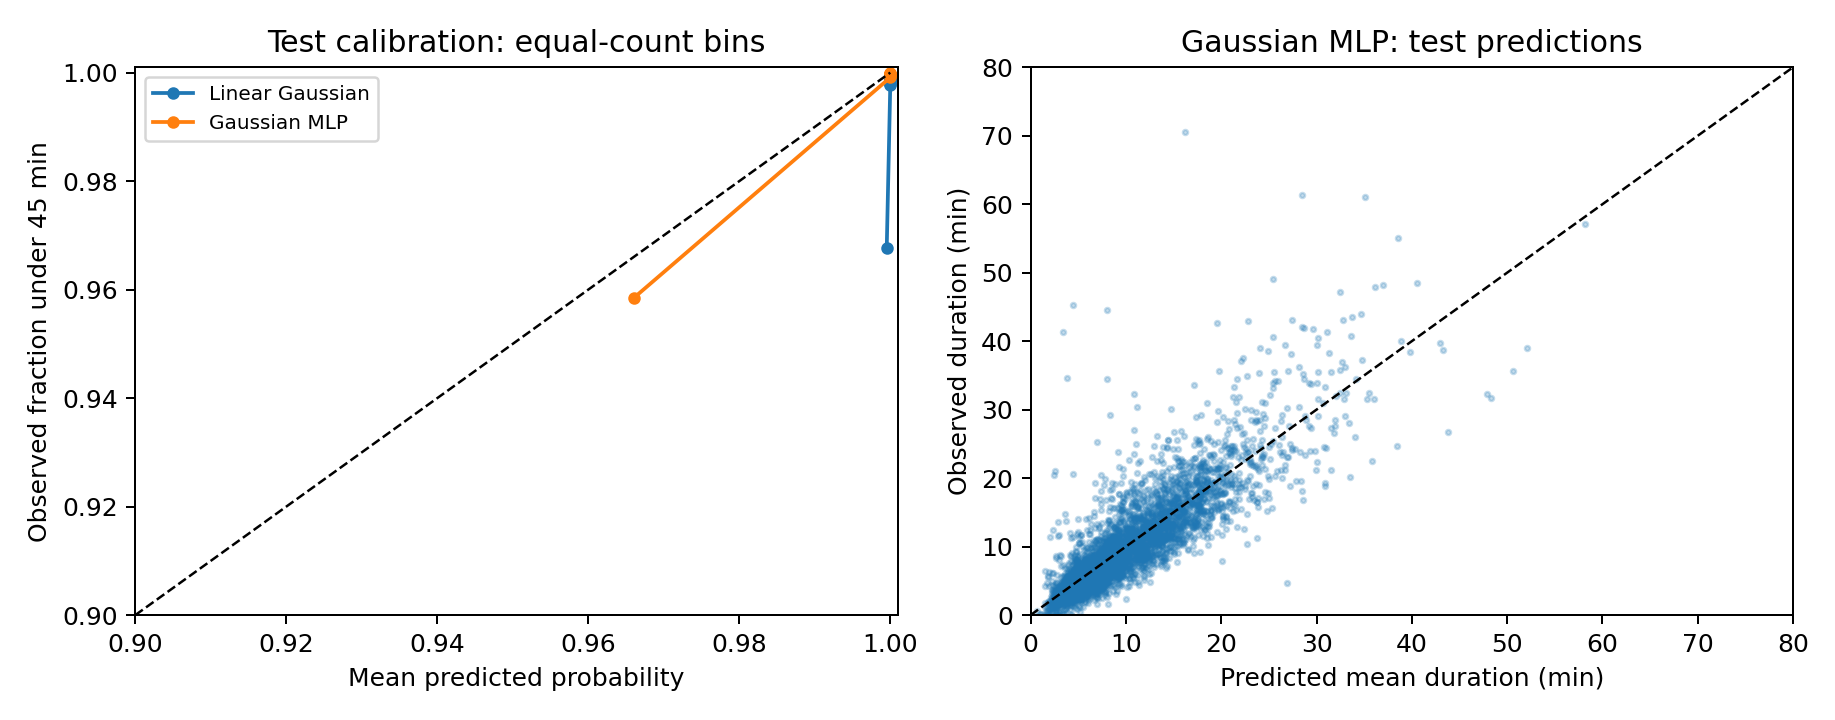
\includegraphics[width=\textwidth]{images/problem1/test_evaluation.png}
\caption{Test calibration in ten equal-count probability bins and a random sample of test mean predictions. Calibration is shown near one because the event is very common.}
\end{figure}
The calibration plot also shows residual probability errors. This random row split measures performance on the supplied distribution and does not evaluate generalization to future time periods.
